\chapter{Thiết kế và xây dựng ứng dụng}
\label{Chapter4-ThietKe}

% ============================================================
\section{Ý tưởng ứng dụng}

Sinh viên Khoa Công nghệ Thông tin tại Trường Đại học Khoa học Tự nhiên (HCMUS) đang phải đối mặt với một khối lượng thông tin học vụ lớn và phân tán: từ chương trình đào tạo, đề cương chi tiết từng môn học, quy chế học vụ đến mạng lưới môn tiên quyết và song hành. Để tìm được câu trả lời cho một câu hỏi đơn giản như ``Mình cần học gì trước khi học Trí tuệ Nhân tạo?'', sinh viên thường phải lần lượt tra cứu qua nhiều tệp PDF rời rạc hoặc chờ đợi giờ tư vấn của giảng viên.

Ý tưởng trung tâm của hệ thống là xây dựng một \textbf{trợ lý học tập thông minh} có khả năng hiểu sâu về toàn bộ kho tri thức học vụ của Khoa. Hệ thống không chỉ trả lời các câu hỏi đơn lẻ mà còn hiểu được mối liên hệ logic giữa các môn học, chuyên ngành và yêu cầu tốt nghiệp, từ đó đưa ra lời tư vấn cá nhân hóa và có căn cứ rõ ràng.

\subsection{Các tình huống sử dụng tiêu biểu}

Tình huống 1: Tra cứu lộ trình môn học.
Sinh viên năm hai đang lập kế hoạch học tập đặt câu hỏi: \textit{``Mình muốn học môn Trí tuệ Nhân tạo thì cần học những môn gì trước?''}. Hệ thống AI Agent phân tích câu hỏi, truy xuất đồ thị tri thức để xác định chuỗi môn tiên quyết, sau đó trả lời chi tiết kèm mã môn học và lộ trình học kỳ gợi ý.

Tình huống 2: Kiểm tra điều kiện tốt nghiệp.
Sinh viên năm bốn hỏi: \textit{``Mình còn thiếu những gì để đủ điều kiện xét tốt nghiệp?''}. Hệ thống đối chiếu hồ sơ học tập cá nhân được lưu trong bộ nhớ dài hạn với quy định chuẩn đầu ra của Khoa, liệt kê các môn còn thiếu và đưa ra gợi ý đăng ký cho học kỳ tiếp theo.

Tình huống 3: Hỏi đáp về quy chế học vụ.
Sinh viên thắc mắc: \textit{``Nếu mình trượt môn tiên quyết thì kỳ sau có được đăng ký môn tiếp theo không?''}. Hệ thống tra cứu quy chế đào tạo tín chỉ của trường, trả lời chính xác với đoạn trích dẫn từ văn bản quy chế tương ứng.

\subsection{Đối tượng người dùng mục tiêu}

Hệ thống hướng tới hai nhóm người dùng chính: \textbf{Sinh viên} Khoa Công nghệ Thông tin tại Trường Đại Học Khoa Học Tự Nhiên, những người cần tra cứu thông tin học vụ và lập kế hoạch học tập.

% ============================================================
\section{Phân tích và đặc tả yêu cầu}

\subsection{Yêu cầu chức năng}

Hệ thống được xác định cần đáp ứng các nhóm chức năng chính được liệt kê trong Bảng~\ref{tab:yc_chuc_nang}.

\begin{table}[H]
	\centering
	\renewcommand{\arraystretch}{1.4}
	\caption{Danh sách yêu cầu chức năng}
	\label{tab:yc_chuc_nang}
	\begin{tabular}{|c|>{\raggedright\arraybackslash}p{4cm}|>{\raggedright\arraybackslash}p{8.5cm}|}
		\hline
		\textbf{STT} & \textbf{Nhóm chức năng} & \textbf{Mô tả} \\ \hline
		1 & Xác thực người dùng & Đăng ký tài khoản, đăng nhập bằng email/mật khẩu, khôi phục mật khẩu qua email. \\ \hline
		2 & Chat với AI Agent & Đặt câu hỏi học vụ bằng ngôn ngữ tự nhiên, nhận câu trả lời có nguồn gốc từ đồ thị tri thức, xem lại lịch sử hội thoại theo phiên. \\ \hline
	\end{tabular}
\end{table}

\subsection{Yêu cầu phi chức năng}

\begin{table}[H]
	\centering
	\renewcommand{\arraystretch}{1.5}
	\caption{Yêu cầu phi chức năng}
	\label{tab:yc_phi_cn}
	\begin{tabular}{|c|l|p{9cm}|}
		\hline
		\textbf{STT} & \textbf{Yêu cầu} & \textbf{Ý nghĩa / Mô tả} \\
		\hline
		1 & Hiệu suất & Giao diện AI Chat phải đảm bảo tải trong vòng $\leq 2$ giây để đảm bảo trải nghiệm người dùng. \\
		\hline
		2 & Khả năng mở rộng & Hệ thống phải mở rộng được để xử lý lượng lớn người dùng và phiên hội thoại đồng thời. \\
		\hline
		3 & Khả dụng & Hệ thống phải hoạt động liên tục với uptime $\geq 99.9\%$/năm. \\
		\hline
		4 & Đáp ứng & Các thao tác cơ bản như đăng nhập, AI Chat phản hồi nhanh (dưới 1 giây). \\
		\hline
		5 & Khả năng sử dụng & UI/UX đơn giản, dễ hiểu, dễ đặt câu hỏi AI. \\
		\hline
	\end{tabular}
\end{table}

\subsection{Danh sách Actor}

Hệ thống xác định một Actor chính tương tác trực tiếp với toàn bộ các chức năng:

\begin{table}[H]
	\centering
	\renewcommand{\arraystretch}{1.5}
	\caption{Danh sách Actor}
	\label{tab:actor}
	\begin{tabular}{|c|l|p{9cm}|}
		\hline
		\textbf{STT} & \textbf{Actor} & \textbf{Ý nghĩa / Ghi chú} \\
		\hline
		1 & Người dùng & Sinh viên trực tiếp sử dụng hệ thống, thao tác các chức năng và gửi phản hồi. \\
		\hline
	\end{tabular}
\end{table}

% ============================================================
\section{Mô hình Use Case}

Hệ thống có một phân hệ chính là \textbf{Sinh viên}, tương tác với hệ thống qua ba chức năng: đăng ký tài khoản, đăng nhập và chat với AI Agent. Sơ đồ Use Case tổng quan được thể hiện tại Hình~\ref{fig:usecase}.

\begin{figure}[H]
	\centering
	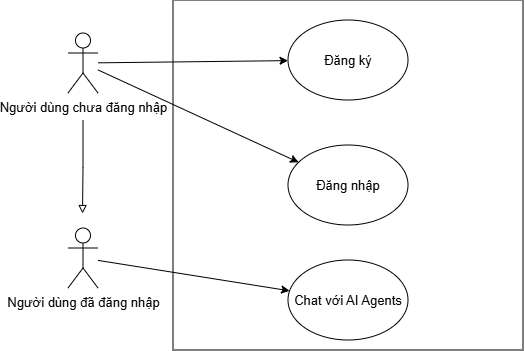
\includegraphics[width=0.8\textwidth]{images/usecase2.drawio.png}
	\caption{Sơ đồ Use Case hệ thống}
	\label{fig:usecase}
\end{figure}

\subsection{Danh sách Use Case}

\begin{table}[H]
	\centering
	\renewcommand{\arraystretch}{1.5}
	\caption{Danh sách Use Case}
	\label{tab:ds_uc}
	\begin{tabular}{|c|p{4.5cm}|p{7cm}|p{2.5cm}|}
		\hline
		\textbf{STT} & \textbf{Tên Use Case} & \textbf{Mô tả} & \textbf{Actor} \\ \hline
		1 & Đăng ký tài khoản & Sinh viên tạo tài khoản mới trên hệ thống. & \multirow{3}{2.5cm}{\centering Sinh viên} \\ \cline{1-3}
		2 & Đăng nhập & Sinh viên đăng nhập bằng email và mật khẩu. & \\ \cline{1-3}
		3 & Chat với AI Agent & Sinh viên đặt câu hỏi học vụ và nhận tư vấn thông minh từ AI. & \\ \hline
	\end{tabular}
\end{table}

\subsection{Đặc tả Use Case}
\setcounter{secnumdepth}{3}
\renewcommand{\arraystretch}{1.4}

\subsubsection{Use Case: Đăng ký tài khoản}
\label{sec:uc-dang-ky}

\begin{longtable}{|>{\raggedright\arraybackslash}p{4.2cm}|>{\raggedright\arraybackslash}p{9.8cm}|}
	\hline
	\textbf{Tên use-case} & Đăng ký tài khoản \\ \hline
	\textbf{Tóm tắt} & Cho phép sinh viên tạo tài khoản mới để sử dụng hệ thống. \\ \hline
	\textbf{Tác nhân} & Sinh viên \\ \hline
	\textbf{Use-case liên quan} & Đăng nhập \\ \hline
	\textbf{Điều kiện tiên quyết} & Email chưa được đăng ký trong hệ thống. \\ \hline
	\textbf{Dòng sự kiện chính} &
	\begin{enumerate}
		\item Sinh viên truy cập trang đăng ký.
		\item Sinh viên nhập họ tên, email và mật khẩu.
		\item Sinh viên xác nhận mật khẩu và đồng ý điều khoản.
		\item Sinh viên nhấn nút \textit{Đăng ký}.
		\item Hệ thống kiểm tra hợp lệ và tạo tài khoản.
		\item Hệ thống chuyển hướng sang trang đăng nhập.
	\end{enumerate} \\ \hline
	\textbf{Dòng sự kiện phụ} & \textbf{A1. Rẽ nhánh tại bước 2, email đã tồn tại:} Hệ thống hiển thị thông báo lỗi và yêu cầu sinh viên sử dụng email khác. \\ \hline
	\textbf{Hậu điều kiện} & Tài khoản được tạo thành công; sinh viên có thể đăng nhập vào hệ thống. \\ \hline
\end{longtable}

\subsubsection{Use Case: Đăng nhập}
\label{sec:uc-dang-nhap}

\begin{longtable}{|>{\raggedright\arraybackslash}p{4.2cm}|>{\raggedright\arraybackslash}p{9.8cm}|}
	\hline
	\textbf{Tên use-case} & Đăng nhập hệ thống \\ \hline
	\textbf{Tóm tắt} & Cho phép sinh viên xác thực danh tính và truy cập vào hệ thống. \\ \hline
	\textbf{Tác nhân} & Sinh viên \\ \hline
	\textbf{Use-case liên quan} & Đăng ký tài khoản, Chat với AI Agent \\ \hline
	\textbf{Điều kiện tiên quyết} & Sinh viên đã có tài khoản được đăng ký trong hệ thống. \\ \hline
	\textbf{Dòng sự kiện chính} &
	\begin{enumerate}
		\item Sinh viên truy cập trang đăng nhập.
		\item Sinh viên nhập email và mật khẩu.
		\item Sinh viên nhấn nút \textit{Đăng nhập}.
		\item Hệ thống xác thực thông tin đăng nhập.
		\item Hệ thống cấp phát JWT token và chuyển hướng đến trang chính.
	\end{enumerate} \\ \hline
	\textbf{Dòng sự kiện phụ} & \textbf{A1. Rẽ nhánh tại bước 4, thông tin không hợp lệ:} Hệ thống hiển thị thông báo lỗi và yêu cầu sinh viên nhập lại.\par\medskip
	\textbf{A2. Quên mật khẩu:} Sinh viên chọn \textit{Quên mật khẩu}, hệ thống gửi email chứa liên kết khôi phục. \\ \hline
	\textbf{Hậu điều kiện} & Sinh viên đăng nhập thành công và có thể sử dụng đầy đủ chức năng hệ thống. \\ \hline
\end{longtable}

\subsubsection{Use Case: Chat với AI Agent}
\label{sec:uc-chat-ai}

\begin{longtable}{|>{\raggedright\arraybackslash}p{4.2cm}|>{\raggedright\arraybackslash}p{9.8cm}|}
	\hline
	\textbf{Tên use-case} & Chat với AI Agent \\ \hline
	\textbf{Tóm tắt} & Sinh viên đặt câu hỏi về học vụ và nhận câu trả lời thông minh từ AI Agent. \\ \hline
	\textbf{Tác nhân} & Sinh viên \\ \hline
	\textbf{Use-case liên quan} & Đăng nhập \\ \hline
	\textbf{Điều kiện tiên quyết} & Sinh viên đã đăng nhập, dịch vụ AI Agent đang hoạt động. \\ \hline
	\textbf{Dòng sự kiện chính} &
	\begin{enumerate}
		\item Sinh viên điều hướng đến phần AI Chat.
		\item Sinh viên nhập câu hỏi liên quan đến học vụ.
		\item Hệ thống chuyển tiếp câu hỏi đến hệ thống AI Agents.
		\item AI Agent phân tích, truy xuất đồ thị tri thức và tạo phản hồi.
		\item Hệ thống hiển thị câu trả lời trong giao diện chat.
		\item Sinh viên có thể đặt câu hỏi tiếp theo, lặp lại bước 2--5.
	\end{enumerate} \\ \hline
	\textbf{Dòng sự kiện phụ} & \textbf{A1. Rẽ nhánh tại bước 5, dịch vụ AI không khả dụng:} Hệ thống hiển thị thông báo lỗi và gợi ý sinh viên thử lại sau.\par\medskip
	\textbf{A2. Câu hỏi ngoài phạm vi:} AI phản hồi rằng câu hỏi nằm ngoài phạm vi hỗ trợ của hệ thống. \\ \hline
	\textbf{Hậu điều kiện} & Sinh viên nhận được câu trả lời, cuộc hội thoại được lưu vào lịch sử phiên. \\ \hline
\end{longtable}

\setcounter{secnumdepth}{3}
\setcounter{tocdepth}{3}

% ============================================================
\section{Kiến trúc hệ thống}

Mô hình kiến trúc tổng thể của hệ thống được đề xuất dựa trên kiến trúc đa tầng (Multi-tier Architecture), nhằm đảm bảo tính tách biệt giữa giao diện người dùng, logic nghiệp vụ và các phân hệ xử lý trí tuệ nhân tạo. Sơ đồ chi tiết được thể hiện tại Hình~\ref{fig:kien_truc_he_thong}.

Sơ lược về kiến trúc được nhóm sử dụng như sau: hệ thống được tổ chức theo mô hình đa tầng gồm bốn tầng chính, trong đó Tầng Giao diện tiếp nhận yêu cầu từ sinh viên và phân phối sang hai luồng xử lý độc lập, Tầng Nghiệp vụ xử lý logic xác thực và nghiệp vụ, Tầng Điều phối AI đảm nhận toàn bộ xử lý trí tuệ nhân tạo, và Tầng Dữ liệu cung cấp hạ tầng lưu trữ chuyên biệt cho từng loại dữ liệu.

\begin{figure}[H]
	\centering
	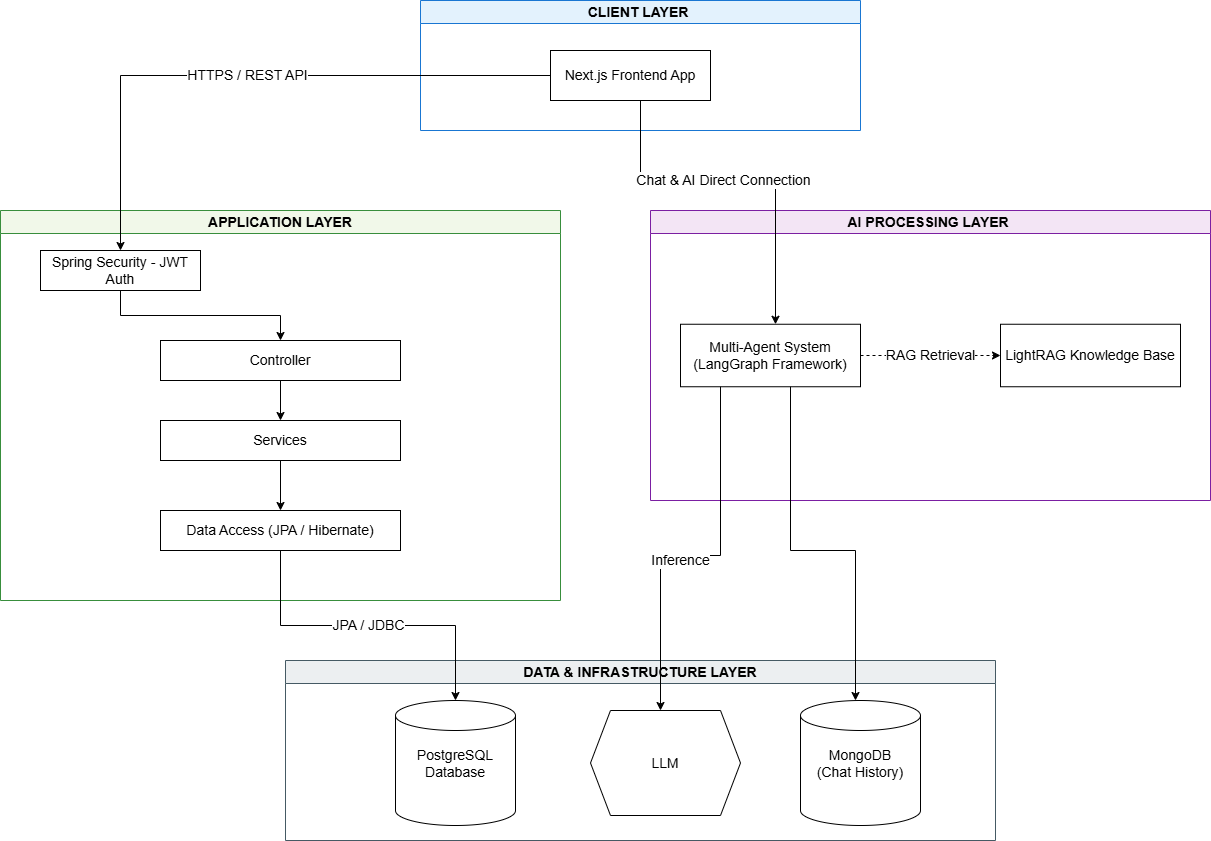
\includegraphics[width=1\textwidth]{images/system_architecture_ver4.drawio.png}
	\caption{Mô hình kiến trúc hệ thống tổng thể}
	\label{fig:kien_truc_he_thong}
\end{figure}

\subsection{Tầng Giao diện (Client Layer)}

Tầng Giao diện được xây dựng trên Next.js, là điểm tiếp xúc duy nhất giữa sinh viên và toàn bộ hệ thống. Khi sinh viên sử dụng ứng dụng, tầng này vận hành hai luồng giao tiếp song song tùy theo tính năng được yêu cầu.

Đối với các tác vụ liên quan đến tài khoản và thông tin cá nhân, ứng dụng giao tiếp với Tầng Nghiệp vụ thông qua giao thức HTTPS và REST API. Đây là luồng truyền thống, đảm bảo tính nhất quán và bảo mật cho các thao tác đọc ghi dữ liệu có cấu trúc.

Đối với tính năng Chat tư vấn học vụ, ứng dụng thiết lập kết nối trực tiếp đến Tầng Điều phối AI (Chat \& AI Direct Connection) mà không đi qua Tầng Nghiệp vụ trung gian. Thiết kế giúp giảm thiểu độ trễ và cho phép hiển thị câu trả lời theo từng phần, giúp mang lại trải nghiệm hội thoại tự nhiên và mượt mà hơn cho người dùng.

\subsection{Tầng Nghiệp vụ (Application Layer)}

Tầng Nghiệp vụ được xây dựng trên Spring Boot, đảm nhận nhiệm vụ xử lý toàn bộ logic nghiệp vụ và kiểm soát luồng dữ liệu giữa các tầng trong hệ thống.

Mọi yêu cầu từ phía Client trước tiên đều phải đi qua lớp bảo mật Spring Security kết hợp với cơ chế xác thực JWT (JSON Web Token). Giúp kiểm tra tính hợp lệ của token và phân quyền truy cập trước khi cho phép yêu cầu đi tiếp vào bên trong hệ thống.

Sau khi xác thực thành công, yêu cầu được định tuyến đến Controller rồi chuyển xuống lớp Services để thực thi logic nghiệp vụ. Lớp Data Access sử dụng Spring Data JPA và Hibernate để ánh xạ đối tượng và giao tiếp với cơ sở dữ liệu PostgreSQL thông qua giao thức JPA/JDBC.

\subsection{Tầng Điều phối AI (AI Processing Layer)}

Tầng Điều phối AI là trung tâm xử lý trí tuệ nhân tạo của hệ thống, tiếp nhận câu hỏi từ sinh viên qua luồng trực tiếp từ Client thông qua Chat \& AI Direct Connection.

Khi nhận được câu hỏi, Multi-Agent System được xây dựng trên LangGraph Framework sẽ điều phối các tác nhân AI chuyên biệt để phân tích ý định câu hỏi, lập kế hoạch trả lời và tổng hợp kết quả. Trước khi sinh ra câu trả lời, hệ thống kích hoạt cơ chế RAG Retrieval để truy xuất các đoạn thông tin liên quan từ LightRAG Knowledge Base, kho tri thức học vụ đã được xây dựng và lập chỉ mục từ tài liệu của Khoa. Việc bổ sung ngữ cảnh từ tri thức thực tế giúp hạn chế tối đa hiện tượng ``ảo giác'' (hallucination) của mô hình ngôn ngữ, đảm bảo câu trả lời có căn cứ rõ ràng.

Sau khi có đầy đủ ngữ cảnh, hệ thống dùng LLM để tạo ra câu trả lời cuối cùng và trả về cho sinh viên.

\subsection{Tầng Dữ liệu và Hạ tầng (Data \& Infrastructure Layer)}

Tầng này gồm ba thành phần chính, mỗi thành phần phục vụ một mục đích riêng biệt.

PostgreSQL được dùng để lưu thông tin tài khoản của sinh viên, bao gồm thông tin đăng nhập, phân quyền và hồ sơ cá nhân. Nhóm chọn PostgreSQL vì hỗ trợ tốt các ràng buộc toàn vẹn dữ liệu, phù hợp với yêu cầu bảo mật cao cho dữ liệu người dùng. Tầng Nghiệp vụ kết nối với PostgreSQL thông qua giao thức JPA/JDBC.

MongoDB lưu lịch sử hội thoại giữa sinh viên và AI Agent theo từng phiên. Do dữ liệu hội thoại không có cấu trúc cố định và cần truy xuất nhanh, MongoDB với cấu trúc tài liệu linh hoạt là lựa chọn phù hợp hơn so với cơ sở dữ liệu quan hệ.

LLM (Large Language Model) là thành phần thực hiện suy luận và sinh ra câu trả lời cuối cùng. Khi Tầng Điều phối AI đã thu thập đủ ngữ cảnh từ Knowledge Graph, yêu cầu Inference được gửi đến LLM để tổng hợp và trả lời cho sinh viên.

% ============================================================
\section{Thiết kế chi tiết các thành phần}

Hệ thống sử dụng ba loại cơ sở dữ liệu với vai trò khác nhau: PostgreSQL lưu thông tin tài khoản người dùng, MongoDB lưu lịch sử hội thoại với AI Agent, và Knowledge Graph (LightRAG) lưu toàn bộ tri thức học vụ phục vụ cho tính năng tư vấn.

\begin{comment}
\subsection{Sơ đồ lớp (Class Diagram)}
% TODO: Thêm hình Class Diagram vào đây khi hoàn thiện
\textit{(Sơ đồ lớp đang được cập nhật.)}

\subsection{Sơ đồ trình tự (Sequence Diagram)}
% TODO: Thêm hình Sequence Diagram vào đây khi hoàn thiện
\textit{(Sơ đồ trình tự đang được cập nhật.)}
\end{comment}

\subsection{Thiết kế cơ sở dữ liệu}

\subsubsection{Cơ sở dữ liệu Quan hệ (PostgreSQL)}

PostgreSQL được dùng để lưu thông tin tài khoản và hồ sơ người dùng trong hệ thống. Cấu trúc quan hệ giúp đảm bảo tính toàn vẹn dữ liệu và hỗ trợ phân quyền chặt chẽ. Sơ đồ tổng quan của cơ sở dữ liệu được thể hiện tại Hình~\ref{fig:mo_hinh_db}.

\begin{figure}[H]
	\centering
	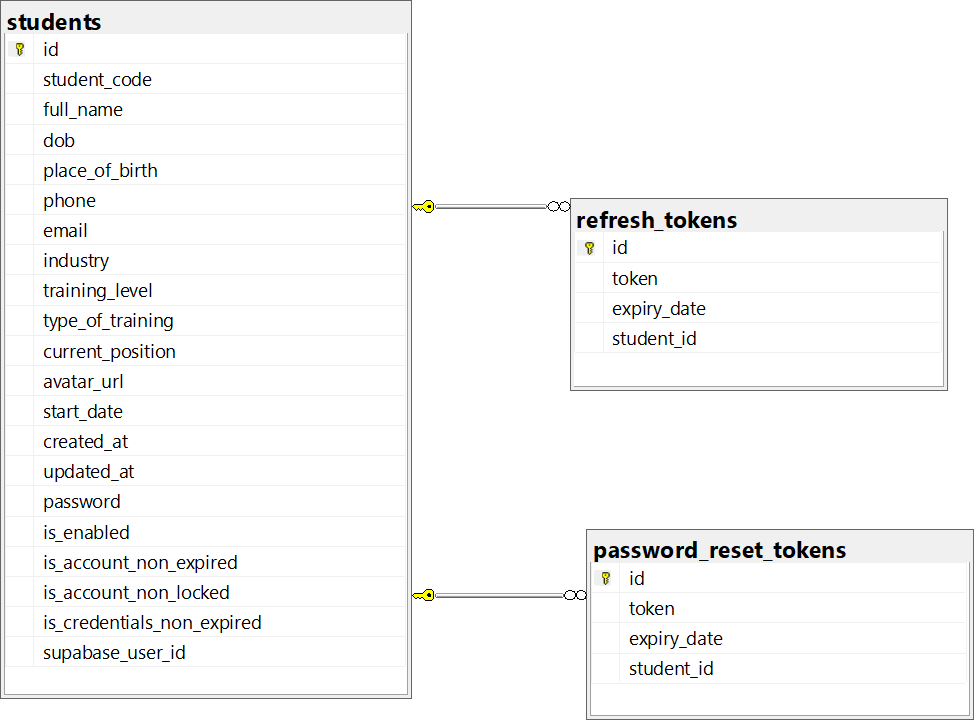
\includegraphics[width=0.85\textwidth]{images/db_diagram.png}
	\caption{Mô hình sơ đồ cơ sở dữ liệu quan hệ người dùng}
	\label{fig:mo_hinh_db}
\end{figure}

{
	\renewcommand{\arraystretch}{1.4}
	\begin{longtable}{|c|>{\raggedright\arraybackslash}p{5.5cm}|>{\raggedright\arraybackslash}p{7.5cm}|}
		\caption{Danh sách các bảng trong cơ sở dữ liệu quan hệ} \label{tab:danh_sach_bang} \\
		\hline
		\textbf{STT} & \textbf{Tên bảng} & \textbf{Ý nghĩa} \\ \hline
		\endfirsthead
		\hline
		\textbf{STT} & \textbf{Tên bảng} & \textbf{Ý nghĩa} \\ \hline
		\endhead
		\hline
		\endfoot
		1 & students & Lưu toàn bộ thông tin hồ sơ người dùng: mã sinh viên, họ tên, ngày sinh, email, mật khẩu, ngành học, trình độ đào tạo và các cờ trạng thái tài khoản (is\_enabled, is\_account\_non\_locked,...). \\ \hline
		2 & refresh\_tokens & Lưu token phiên làm việc (token, expiry\_date) để duy trì trạng thái đăng nhập mà không cần xác thực lại. \\ \hline
		3 & password\_reset\_tokens & Lưu token bảo mật (token, expiry\_date) dùng trong quy trình đặt lại mật khẩu. \\ \hline
	\end{longtable}
}

\textbf{Ràng buộc Khóa ngoại}

{
	\renewcommand{\arraystretch}{1.4}
	\begin{longtable}{|c|>{\raggedright\arraybackslash}p{5cm}|>{\raggedright\arraybackslash}p{2.5cm}|>{\raggedright\arraybackslash}p{2cm}|>{\raggedright\arraybackslash}p{1.5cm}|}
		\caption{Mô tả khóa ngoại của các bảng trong CSDL quan hệ} \label{tab:khoa_ngoai} \\
		\hline
		\textbf{STT} & \textbf{Tên Bảng} & \textbf{Tên cột} & \textbf{Bảng tham chiếu} & \textbf{Cột tham chiếu} \\ \hline
		\endfirsthead
		\hline
		\textbf{STT} & \textbf{Tên Bảng} & \textbf{Tên cột} & \textbf{Bảng tham chiếu} & \textbf{Cột tham chiếu} \\ \hline
		\endhead
		\hline
		\endfoot
		1 & refresh\_tokens & student\_id & students & id \\ \hline
		2 & password\_reset\_tokens & student\_id & students & id \\ \hline
	\end{longtable}
}

\subsubsection{Cơ sở dữ liệu Phi cấu trúc (MongoDB)}
Để phục vụ cho tác nhân duy trì bộ nhớ dài hạn (Long-term Memory Agent) và quản lý trạng thái luồng suy luận trong kiến trúc LangGraph, hệ thống sử dụng MongoDB. Dữ liệu được tổ chức linh hoạt để lưu trữ lịch sử hội thoại và các điểm kiểm soát (checkpoints) của AI Agent.

{
	\renewcommand{\arraystretch}{1.4}
	\begin{longtable}{|c|p{4.5cm}|p{8.5cm}|}
		\caption{Danh sách các Collection trong cơ sở dữ liệu hcmus\_langgraph} \label{tab:mongo_collections} \\
		\hline
		\textbf{STT} & \textbf{Tên Collection} & \textbf{Ý nghĩa dữ liệu thực tế} \\ \hline
		\endfirsthead
		\hline
		\textbf{STT} & \textbf{Tên Collection} & \textbf{Ý nghĩa dữ liệu thực tế} \\ \hline
		\endhead
		\hline
		\endfoot
		1 & session\_info & Lưu trữ thông tin định danh của phiên chat bao gồm: session\_id, user\_id, tiêu đề cuộc hội thoại và thời gian cập nhật gần nhất. \\ \hline
		2 & long\_term\_memory & Lưu trữ các tri thức hoặc thông tin quan trọng được đúc kết từ các cuộc hội thoại cũ để AI Agent sử dụng cho các lần tương tác sau. \\ \hline
		3 & checkpoints & Lưu trữ trạng thái hiện tại (State) của luồng LangGraph, cho phép hệ thống phục hồi lại đúng bước đang xử lý khi có lỗi hoặc ngắt quãng. \\ \hline
		4 & checkpoint\_writes & Ghi lại nhật ký các thay đổi của trạng thái Agent qua từng bước trong luồng điều phối. \\ \hline
	\end{longtable}
}

\subsubsection{Cơ sở dữ liệu Đồ thị (Knowledge Graph)}
Hệ thống sử dụng LightRAG để xây dựng đồ thị tri thức học vụ, phục vụ lưu trữ thông tin phức tạp với nhiều mối quan hệ đan xen. Thay vì cấu trúc bảng (Table), dữ liệu được biểu diễn dưới dạng Thực thể (Nodes) và Mối quan hệ (Edges/Relationships), lưu trữ trong Neo4j.

Cấu trúc đồ thị tri thức được phân tích theo hai lớp: lớp khái niệm (logical view) thể hiện ngữ nghĩa các loại thực thể và quan hệ, và lớp lưu trữ vật lý (physical view) phản ánh cách triển khai thực tế trong Neo4j.

\setcounter{secnumdepth}{4}
\setcounter{tocdepth}{4}

\paragraph{Lớp khái niệm (logical view)}
Hình~\ref{fig:kg-concept-model} thể hiện mô hình khái niệm các loại thực thể và quan hệ chính trong đồ thị tri thức học vụ.

\begin{figure}[H]
\centering
\begin{tikzpicture}[
	docnode/.style={rectangle, rounded corners=6pt,
		draw=blue!50!violet!80, fill=blue!15!violet!25,
		minimum width=4.3cm, minimum height=1.3cm,
		align=center, inner sep=7pt},
	coursenode/.style={rectangle, rounded corners=6pt,
		draw=teal!80, fill=teal!30,
		minimum width=4.2cm, minimum height=1.3cm,
		align=center, inner sep=7pt},
	outcomenode/.style={rectangle, rounded corners=6pt,
		draw=orange!70!red!60, fill=orange!35!red!20,
		minimum width=4.3cm, minimum height=1.3cm,
		align=center, inner sep=7pt},
	programnode/.style={rectangle, rounded corners=6pt,
		draw=gray!65, fill=gray!20,
		minimum width=5.2cm, minimum height=1.3cm,
		align=center, inner sep=7pt},
	rel/.style={-Stealth, thick, draw=black!65},
	lbl/.style={fill=white, inner sep=1.5pt, font=\scriptsize},
]

% ==================== Nodes ====================
\node[docnode]     (vbqd) at (0.0, 5.0) {\textbf{Văn bản quy định}\\{\small Quy chế, đề cương}};
\node[outcomenode] (cdr)  at (10.0, 5.0) {\textbf{Chuẩn đầu ra}\\{\small Kỹ năng, kiến thức}};

\node[coursenode]  (mhA)  at (0.0, 2.0) {\textbf{Môn học A}\\{\small Học phần tiên quyết}};
\node[coursenode]  (mhB)  at (6.6, 2.0) {\textbf{Môn học B}\\{\small Học phần, tín chỉ}};

\node[programnode] (ctdt) at (6.6, -1.0) {\textbf{Chương trình đào tạo}\\{\small Ngành, chuyên ngành}};

% ==================== Relationships ====================
\draw[rel] (vbqd.south east) -- (mhB.north west);
\node[lbl] at (3.6, 3.65) {QUY ĐỊNH};

% \draw[rel] (mhB.north east) to[out=35,in=-90] (cdr.south);
\draw[rel] (mhB.north east) -- (cdr.south);
\node[lbl] at (8.35, 3.55) {ĐÁP ỨNG};

\draw[rel] (mhA.east) -- (mhB.west);
\node[lbl] at (3.3, 2.45) {TIÊN QUYẾT};

\draw[rel] (mhB.south) -- (ctdt.north);
\node[lbl] at (7.5, 0.45) {THUỘC};

% ==================== Legend ====================
\begin{scope}[shift={(1.2,-3.2)}]
	\filldraw[draw=blue!50!violet!80, fill=blue!15!violet!25] (0.0, 0.0) circle (0.18cm);
	\node[right=0.08cm] at (0.20, 0.0) {\small Văn bản quy định};

	\filldraw[draw=teal!80, fill=teal!30] (5.0, 0.0) circle (0.18cm);
	\node[right=0.08cm] at (5.20, 0.0) {\small Môn học};

	\filldraw[draw=orange!70!red!60, fill=orange!35!red!20] (0.0, -0.8) circle (0.18cm);
	\node[right=0.08cm] at (0.20, -0.8) {\small Chuẩn đầu ra};

	\filldraw[draw=gray!65, fill=gray!20] (5.0, -0.8) circle (0.18cm);
	\node[right=0.08cm] at (5.20, -0.8) {\small Chương trình đào tạo};
\end{scope}

\end{tikzpicture}
\caption{Mô hình khái niệm các loại thực thể và quan hệ chính trong đồ thị tri thức học vụ}
\label{fig:kg-concept-model}
\end{figure}

Về mặt khái niệm, đồ thị gồm bốn nhóm thực thể chính. Môn học là thực thể trung tâm, lưu các học phần cùng thông tin tín chỉ, các môn có thể liên kết tiên quyết với nhau qua quan hệ TIÊN QUYẾT. Chương trình đào tạo nhóm các môn học theo ngành và chuyên ngành qua quan hệ THUỘC. Chuẩn đầu ra mô tả các kỹ năng, kiến thức cần đạt qua quan hệ ĐÁP ỨNG. Văn bản quy định gồm quy chế và đề cương là nguồn gốc tri thức của hệ thống, liên kết qua quan hệ QUY ĐỊNH.

\paragraph{Lớp lưu trữ vật lý (physical view)}
Về mặt triển khai trong Neo4j, toàn bộ các quan hệ đều được lưu dưới một relationship type duy nhất là DIRECTED, ngữ nghĩa cụ thể được mã hóa trong thuộc tính keywords do mô hình ngôn ngữ lớn sinh ra trong quá trình trích xuất.

Mỗi thực thể được lưu dưới dạng một node với hai nhãn: nhãn \textit{workspace} (phân vùng dữ liệu, ví dụ base) và nhãn \textit{entity\_type} (phân loại ngữ nghĩa, ví dụ Course, Concept). Bảng~\ref{tab:kg-node-props} liệt kê các thuộc tính của node.

\begin{table}[H]
	\centering
	\renewcommand{\arraystretch}{1.4}
	\caption{Thuộc tính của node thực thể trong Knowledge Graph (Neo4j)}
	\label{tab:kg-node-props}
	\begin{tabular}{|>{\raggedright\arraybackslash}p{3.2cm}|>{\raggedright\arraybackslash}p{1.6cm}|>{\raggedright\arraybackslash}p{8.5cm}|}
		\hline
		\textbf{Thuộc tính} & \textbf{Kiểu} & \textbf{Mô tả \& Ví dụ} \\ \hline
		entity\_id   & string  & Tên thực thể (chuẩn hóa chữ thường). VD: "cơ sở dữ liệu" \\ \hline
		entity\_type & string  & Loại thực thể do LLM phân loại. VD: "Course" \\ \hline
		description  & string  & Mô tả tổng hợp từ nhiều tài liệu, các đoạn nối bằng <SEP>. VD: "Môn học về quản lý dữ liệu<SEP>Nghiên cứu SQL" \\ \hline
		source\_id   & string  & Danh sách ID chunk nguồn, nối bằng <SEP>. VD: "chunk-abc123<SEP>chunk-def456" \\ \hline
		file\_path   & string  & Tài liệu gốc chứa thực thể, nhiều giá trị nối bằng <SEP>. VD: "chuong\_trinh.pdf<SEP>decuong.pdf" \\ \hline
		created\_at  & integer & Unix timestamp thời điểm tạo. VD: 1719571200 \\ \hline
		truncate     & string  & Trạng thái giới hạn source\_id: "" hoặc "KEEP Old" \\ \hline
	\end{tabular}
\end{table}

Trường hợp đặc biệt là quan hệ đồng nhất thực thể, được biểu diễn bằng cùng type DIRECTED nhưng với keywords = "SAME\_AS". Bảng~\ref{tab:kg-edge-props} mô tả các thuộc tính của relationship.

\begin{table}[H]
	\centering
	\renewcommand{\arraystretch}{1.4}
	\caption{Thuộc tính của relationship trong Knowledge Graph (Neo4j)}
	\label{tab:kg-edge-props}
	\begin{tabular}{|>{\raggedright\arraybackslash}p{3.2cm}|>{\raggedright\arraybackslash}p{1.6cm}|>{\raggedright\arraybackslash}p{8.5cm}|}
		\hline
		\textbf{Thuộc tính} & \textbf{Kiểu} & \textbf{Mô tả \& Ví dụ} \\ \hline
		keywords     & string  & Từ khóa mô tả bản chất quan hệ, do LLM sinh ra. VD: "tiên quyết, học trước" hoặc "SAME\_AS" \\ \hline
		description  & string  & Diễn giải quan hệ theo ngữ cảnh tài liệu, nhiều mô tả nối bằng <SEP>. VD: "Nhập môn Lập trình là môn tiên quyết của Cơ sở dữ liệu" \\ \hline
		weight       & float   & Trọng số quan hệ, tỉ lệ với số lần quan hệ xuất hiện. VD: 3.0 \\ \hline
		source\_id   & string  & ID các chunk nguồn hỗ trợ quan hệ này. VD: "chunk-abc123" \\ \hline
		file\_path   & string  & Tài liệu gốc của quan hệ. VD: "chuong\_trinh.pdf" \\ \hline
		created\_at  & integer & Unix timestamp thời điểm tạo. VD: 1719571200 \\ \hline
	\end{tabular}
\end{table}

\begin{comment}
\paragraph{Phân loại thực thể trong corpus học thuật HCMUS.}
Thay vì sử dụng schema cố định, hệ thống áp dụng phương pháp phân loại
\textit{schema-free}: danh sách entity type được cấu hình riêng cho từng
domain và truyền vào prompt của mô hình ngôn ngữ lớn khi trích xuất.
Đối với corpus học thuật của trường Đại học Khoa học Tự nhiên, hệ thống
sử dụng 19 loại thực thể sau:

\begin{table}[H]
	\centering
	\renewcommand{\arraystretch}{1.4}
	\caption{Danh sách entity type cấu hình cho corpus học thuật HCMUS}
	\label{tab:entity-types-datn}
	\begin{tabular}{|>{\raggedright\arraybackslash}p{4.0cm}|>{\raggedright\arraybackslash}p{4.0cm}|>{\raggedright\arraybackslash}p{4.5cm}|}
		\hline
		\multicolumn{3}{|l|}{\textbf{Các loại thực thể (entity type) được định nghĩa}} \\ \hline
		\texttt{Course}            & \texttt{Major}              & \texttt{KnowledgeBlock} \\ \hline
		\texttt{Program}           & \texttt{Department}         & \texttt{Concept} \\ \hline
		\texttt{Skill}             & \texttt{Policy}             & \texttt{LearningOutcome} \\ \hline
		\texttt{AssessmentMethod}  & \texttt{Topic}              & \texttt{Instructor} \\ \hline
		\texttt{Semester}          & \texttt{TotalCredits}       & \texttt{SelfStudyHours} \\ \hline
		\texttt{TrainingTime}      & \texttt{InstructionalTime}  & \texttt{author} \\ \hline
		\texttt{yearofpublication} & \multicolumn{2}{>{\raggedright\arraybackslash}p{9.0cm}|}{\textit{(không khớp loại nào)} $\rightarrow$ \texttt{Other}} \\ \hline
	\end{tabular}
\end{table}
\end{comment}

Hình~\ref{fig:kg-subgraph-example} minh họa một đoạn đồ thị tri thức được
trích xuất từ đề cương môn học, trong đó Cơ sở dữ liệu là thực thể canonical,
CSDL và CSC10002 là alias liên kết qua quan hệ SAME\_AS,
các mũi tên thể hiện quan hệ ngữ nghĩa với nhãn keywords tương ứng.

\begin{figure}[H]
\centering
\resizebox{\linewidth}{!}{%
\begin{tikzpicture}[
    every node/.style={font=\small},
    coursenode/.style={
        rectangle, rounded corners=5pt,
        draw=blue!70, fill=blue!10,
        minimum width=4.2cm, minimum height=1.0cm,
        align=center, inner sep=6pt
    },
    conceptnode/.style={
        rectangle, rounded corners=5pt,
        draw=teal!70, fill=teal!8,
        minimum width=3.4cm, minimum height=1.0cm,
        align=center, inner sep=5pt
    },
    deptnode/.style={
        rectangle, rounded corners=5pt,
        draw=gray!60, fill=gray!8,
        minimum width=3.4cm, minimum height=1.0cm,
        align=center, inner sep=5pt
    },
    aliasnode/.style={
        rectangle, rounded corners=4pt,
        draw=blue!40, fill=blue!4,
        minimum width=3.4cm, minimum height=0.9cm,
        align=center, inner sep=5pt
    },
    instrnode/.style={
        rectangle, rounded corners=5pt,
        draw=orange!60, fill=orange!7,
        minimum width=3.4cm, minimum height=1.0cm,
        align=center, inner sep=5pt
    },
    rel/.style={-Stealth, thick, draw=blue!55},
    sameas/.style={-Stealth, thick, dashed, draw=orange!70},
    lbl/.style={font=\small\itshape, fill=white, inner sep=2pt},
    slbl/.style={font=\small, color=orange!80!black, fill=white, inner sep=3pt},
]

% ── Hàng trên: prerequisite courses ──
\node[coursenode] (nlp)  at (1.0, 5.0) {Nhập môn Lập trình\\{\small :Course}};
\node[coursenode] (ctdl) at (7.0, 5.0) {Cấu trúc dữ liệu\\{\small :Course}};

% ── Hàng giữa: central node ──
\node[coursenode, draw=blue!90, fill=blue!20, font=\small, minimum width=5.5cm]
    (csdl) at (7.0, 2.5) {Cơ sở dữ liệu\\{\small :Course \quad entity\_id="cơ sở dữ liệu"}};

% ── Alias trái: CSDL ──
\node[aliasnode] (alias1) at (-1.5, 2.5) {CSDL\\{\small :Course}};

% ── Alias phải: CSC10002 ──
\node[aliasnode] (alias2) at (14.5, 2.5) {CSC10002\\{\small :Course}};

% ── Hàng dưới: related nodes ──
\node[instrnode]   (gv)   at (1.0, 0.0)  {Nguyễn Văn A\\{\small :Instructor}};
\node[deptnode]    (khoa) at (7.0, 0.0)  {Khoa CNTT\\{\small :Department}};
\node[conceptnode] (sql)  at (13.0, 0.0) {SQL\\{\small :Concept}};

% ── Quan hệ ngữ nghĩa ──
\draw[rel] (nlp.south)       -- node[lbl, left=2pt]{tiên quyết của}  (csdl.north west);
\draw[rel] (ctdl.south)      -- node[lbl, right=2pt]{tiên quyết của} (csdl.north);
\draw[rel] (csdl.south west) -- node[lbl, left=2pt]{giảng dạy bởi}   (gv.north);
\draw[rel] (csdl.south)      -- node[lbl, right=2pt]{thuộc}           (khoa.north);
\draw[rel] (csdl.south east) -- node[lbl, right=2pt]{sử dụng}         (sql.north);
\draw[rel] (alias2.west)     -- node[lbl, above=3pt]{mã học phần của}    (csdl.east);

% ── SAME_AS edge ──
\draw[sameas] (alias1.east) -- node[slbl, above=5pt]{SAME\_AS} (csdl.west);

\end{tikzpicture}
}%
\caption{Ví dụ subgraph trích xuất từ đề cương môn học trong Knowledge Graph}
\label{fig:kg-subgraph-example}
\end{figure}

\setcounter{secnumdepth}{3}
\setcounter{tocdepth}{3}

\subsection{Kiến trúc triển khai lưu trữ cho LightRAG}
\label{sec:lightrag_storage}

\indent Để vận hành hiệu quả các quy trình lập chỉ mục và truy xuất tri thức, hệ thống LightRAG được triển khai với kiến trúc lưu trữ hỗn hợp gồm bốn thành phần chuyên biệt. Sơ đồ tổng quan được thể hiện tại Hình~\ref{fig:storage_deployment}.

\begin{figure}[H]
	\centering
	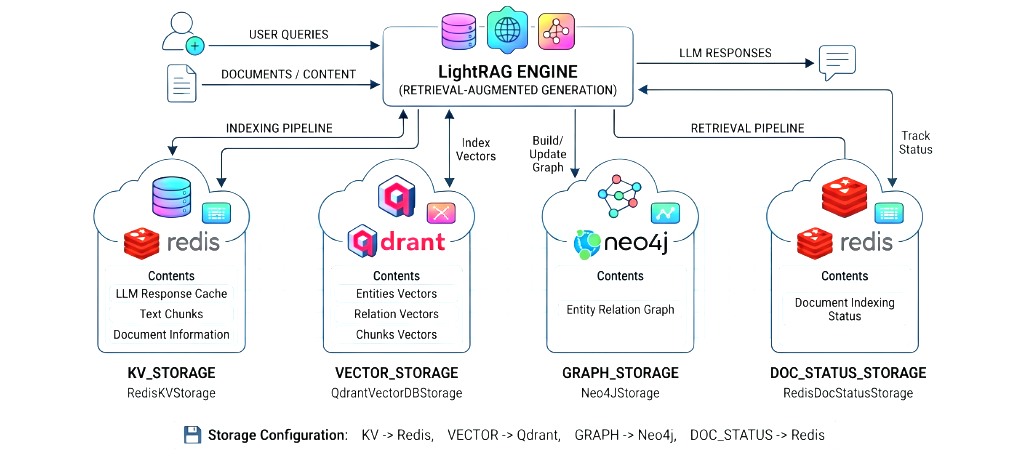
\includegraphics[width=1\textwidth]{images/storage_deployment_overview_nobg.png}
	\caption{Tổng quan kiến trúc lưu trữ và triển khai LightRAG}
	\label{fig:storage_deployment}
\end{figure}

\indent Thành phần thứ nhất là \textbf{KV\_STORAGE}, triển khai trên Redis, chịu trách nhiệm lưu trữ bộ nhớ đệm phản hồi LLM, các đoạn văn bản đã phân mảnh và siêu dữ liệu tài liệu gốc. Thành phần thứ hai là \textbf{VECTOR\_STORAGE}, triển khai trên Qdrant, lưu trữ vector nhúng của thực thể, quan hệ và đoạn văn bản để phục vụ tìm kiếm ngữ nghĩa. Thành phần thứ ba là \textbf{GRAPH\_STORAGE}, triển khai trên Neo4j, lưu toàn bộ cấu trúc đồ thị tri thức với ngôn ngữ truy vấn Cypher. Thành phần thứ tư là \textbf{DOC\_STATUS\_STORAGE}, triển khai trên Redis, theo dõi trạng thái lập chỉ mục từng tài liệu để tránh xử lý trùng lặp.

\begin{table}[H]
	\centering
	\renewcommand{\arraystretch}{1.4}
	\caption{Các thành phần lưu trữ trong kiến trúc LightRAG}
	\label{tab:storage_mapping}
	\footnotesize
	\begin{tabular}{|>{\raggedright\arraybackslash}p{4.5cm}|>{\raggedright\arraybackslash}p{1.5cm}|>{\raggedright\arraybackslash}p{4.5cm}|>{\raggedright\arraybackslash}p{3cm}|}
		\hline
		\textbf{Thành phần} & \textbf{Công nghệ} & \textbf{Lớp triển khai} & \textbf{Dữ liệu lưu trữ} \\ \hline
		KV\_STORAGE & Redis & RedisKVStorage & LLM Response Cache, Text Chunks, Document Information \\ \hline
		VECTOR\_STORAGE & Qdrant & QdrantVectorDBStorage & Entities Vectors, Relation Vectors, Chunks Vectors \\ \hline
		GRAPH\_STORAGE & Neo4j & Neo4JStorage & Entity Relation Graph \\ \hline
		DOC\_STATUS\_STORAGE & Redis & RedisDocStatusStorage & Document Indexing Status \\ \hline
	\end{tabular}
\end{table}

% ============================================================
\clearpage
\section{Thiết kế giao diện}

\subsection{Màn hình AI Chat}

\begin{figure}[H]
	\centering
	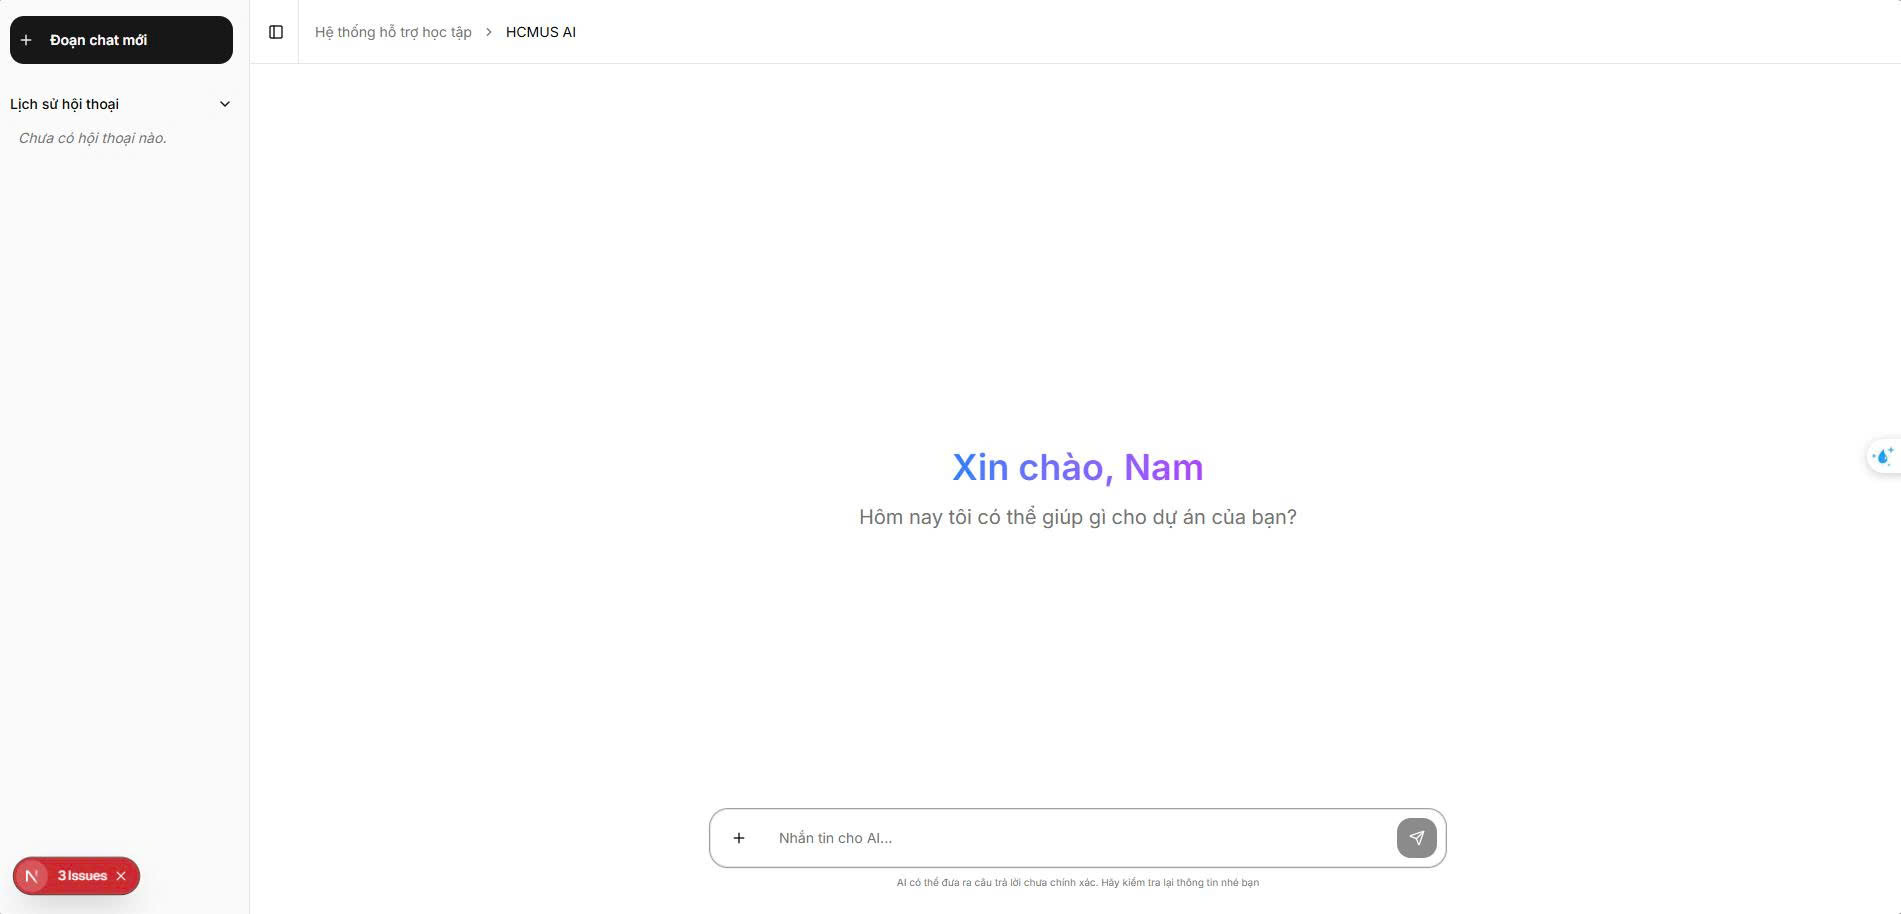
\includegraphics[width=1\textwidth]{images/aichat.jpg}
	\caption{Giao diện Màn hình AI Chat}
	\label{fig:ui_ai_chat}
\end{figure}

\textbf{Mục đích:} Cung cấp không gian trò chuyện trực tiếp giữa sinh viên và AI Agent để được tư vấn thông tin học vụ, lộ trình môn học và quy chế đào tạo.

Bao gồm:
\begin{enumerate}
	\item Thanh lịch sử hội thoại (bên trái)
	\item Khu vực hiển thị hội thoại (trung tâm)
	\item Ô nhập câu hỏi và nút gửi (phía dưới)
\end{enumerate}

\textbf{Cách sử dụng:}
\begin{itemize}
	\item \textbf{Để đặt câu hỏi cho AI Agent:}
	\begin{enumerate}
		\item Nhập câu hỏi vào ô nhập liệu ở phía dưới màn hình.
		\item Nhấn nút gửi.
		\item Hệ thống phân tích câu hỏi, truy xuất đồ thị tri thức và trả về câu trả lời chi tiết trong khu vực hội thoại.
	\end{enumerate}
	\item \textbf{Để xem lại lịch sử hội thoại:}
	\begin{enumerate}
		\item Chọn phiên hội thoại tại thanh danh sách bên trái.
		\item Hệ thống hiển thị toàn bộ nội dung của phiên đó.
	\end{enumerate}
\end{itemize}
